\begin{surferPage}[Chmutov-Octic]{A Chmutov Octic}
    %An eye-catching feature of Chmutov's octic $\text{Chm}_{d}, \ d=8,$
		Gledaju\'{c}i Chmutovljevu oktiku $\text{Chm}_{d}, \ d=8,$
    %is its symmetry.
		uo\v{c}avamo njenu simetriju.
    %This can also be seen by inspecting the equation:
		Promotrimo jednad\v{z}bu:
    \[\text{Chm}_{d}\colon T_d(x) + T_d(y) + T_d(z) + 1 = 0,\]
    % where $T_d$ is the so--called Tchebychev polynomial (left picture).
		gdje je $T_d$ Tchebychevljev polinom (lijeva slika).
    %The curve $T_8(x)+T_8(y)=0$ is depicted on the right:
		Krivulja $T_8(x)+T_8(y)=0$ je prikazana na desnoj strani:
    
     \begin{center}
      \begin{tabular}{c@{\quad}c}
        \begin{tabular}{c}
          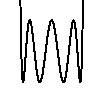
\includegraphics[height=1.75cm]{./../../common/images/Tcheb_008.pdf}
        \end{tabular}    
        &
        \begin{tabular}{c}
          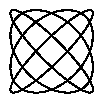
\includegraphics[height=1.75cm]{./../../common/images/Tcheb_2d_008.pdf}
        \end{tabular}    
      \end{tabular}
    \end{center}
    \vspace{-0.3cm}
    %The steps required of going from these pictures to the shape of the surface in the
		Iz ovih slika nije te\v{s}ko do\'{c}i do oblika plohe u
    %interactive viewer are not very difficult.
		interaktivnom pregledniku.


%These equations where given by S.V.\ Chmutov in the early 80s.
Do navedenih jednad\v{z}bi do\v{s}ao je S.V.\ Chmutov ranih 80.-ih.
    %At that time, they constituted the world record for $\mu(d)$ most $d$.
		U to vrijeme je svjetski rekord za $\mu(d)$ bio $d$.
    %In the 90s, Chmutov improved his own record, and in 2005, S.~Breske,
		90.-ih je Chmutov popravio svoj rekord, a 2005. su S.~Breske, 
    %O.~Labs and D.~van~Straten adapted this construction to yield real
		O.~Labs i D.~van~Straten prilagodili njegovu konstrukciju da bi dobili
    %surfaces with only real singularities.
		realne plohe koje imaju samo realne singularitete.
\end{surferPage}